\documentclass[twoside,a4paper]{article}
\usepackage{geometry}
\geometry{margin=1.5cm, vmargin={0pt,1cm}}
\setlength{\topmargin}{-1cm}
\setlength{\paperheight}{29.7cm}
\setlength{\textheight}{25.3cm}

% useful packages.
\usepackage{amsfonts}
\usepackage{amsmath}
\usepackage{amssymb}
\usepackage{amsthm}
\usepackage{enumerate}
\usepackage{graphicx}[H]
\usepackage{multicol}
\usepackage{fancyhdr}
\usepackage{layout}
\usepackage{float}
\usepackage{listings}
\usepackage{listings}
\lstset{numbers=left}

% some common command
\newcommand{\dif}{\mathrm{d}}
\newcommand{\avg}[1]{\left\langle #1 \right\rangle}
\newcommand{\difFrac}[2]{\frac{\dif #1}{\dif #2}}
\newcommand{\pdfFrac}[2]{\frac{\partial #1}{\partial #2}}
\newcommand{\OFL}{\mathrm{OFL}}
\newcommand{\UFL}{\mathrm{UFL}}
\newcommand{\fl}{\mathrm{fl}}
\newcommand{\op}{\odot}
\newcommand{\Eabs}{E_{\mathrm{abs}}}
\newcommand{\Erel}{E_{\mathrm{rel}}}

\begin{document}

\pagestyle{fancy}
\fancyhead{}
\lhead{Jovi Wong(3180104829)}
\chead{Math Software \#day5}
\rhead{2020/7/10}


\section*{I. Exercise in Handout}

\subsection*{I-a. Divide image by K-mean algorithm} 
\begin{figure}[H]
\centering
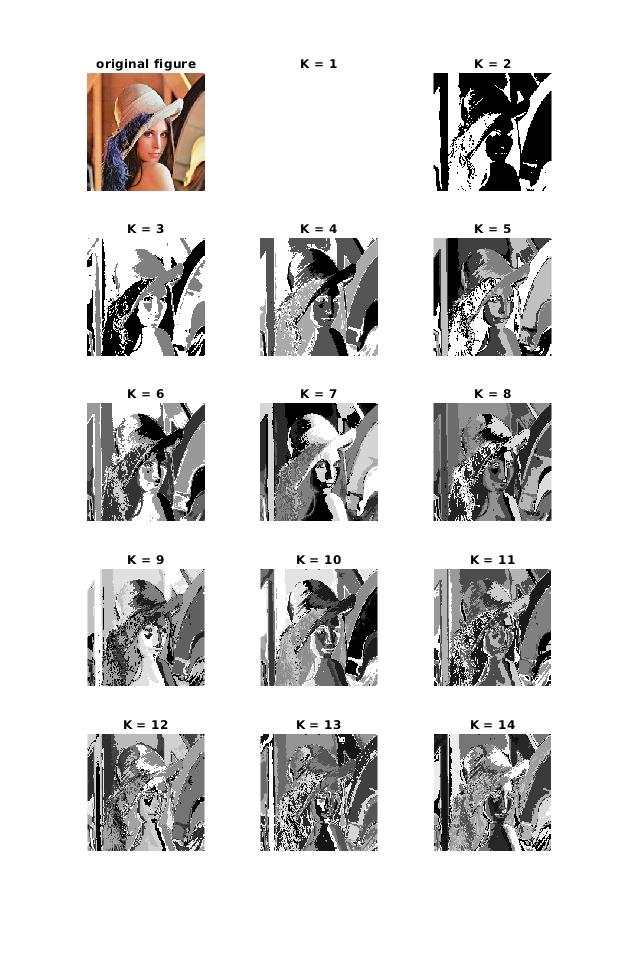
\includegraphics[width=5.5in]{kmeanlena1.jpg}
\end{figure}


\subsection*{I-b. Aggression for Blood pressure} 
\begin{figure}[H]
\centering
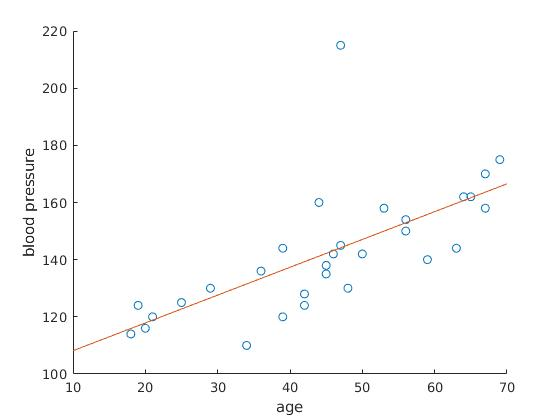
\includegraphics[width=6in]{age2blood.jpg}
\end{figure}

\begin{figure}[H]
\centering
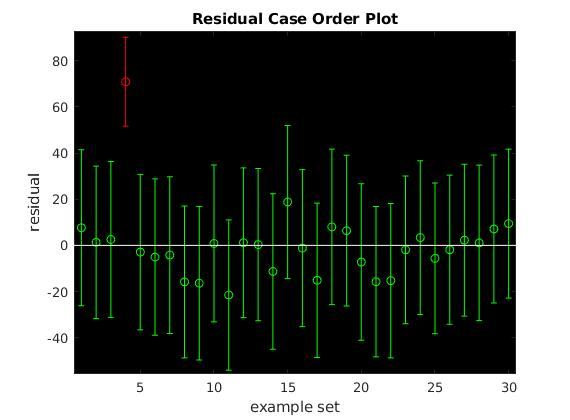
\includegraphics[width=6in]{resdual.jpg}
\end{figure}
We can get coefficients of each parameter by linear aggression as follwing
\begin{equation}
BloodPressure = 45.3636 + 0.3604\times Age + 3.0906\times Weight + 11.8246\times Ciggretta
\end{equation}
\subsection*{I-c. Regress without abnormal data}
\begin{figure}[H]
\centering
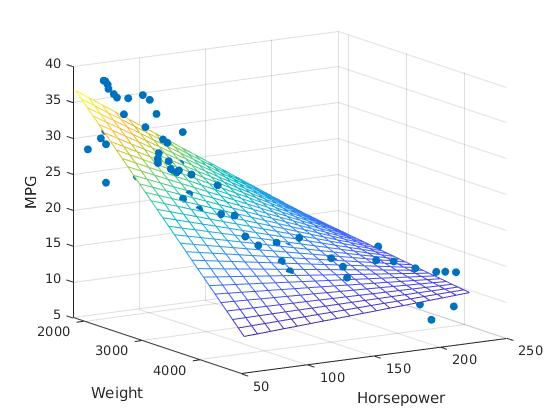
\includegraphics[width=6in]{newregress.jpg}
\end{figure}

\begin{figure}[H]
\centering
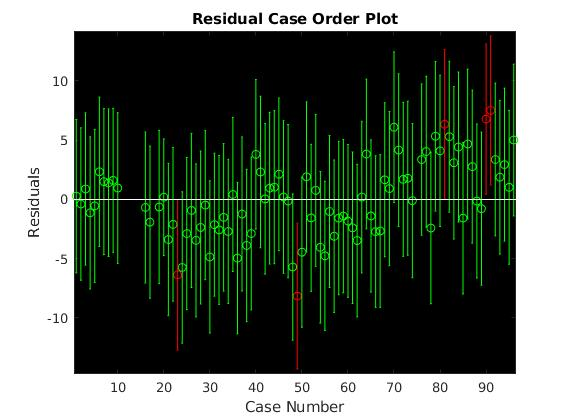
\includegraphics[width=6in]{resnew.jpg}
\end{figure}


\section*{II. Face Recognition by SVM}
\begin{figure}[H]
\centering
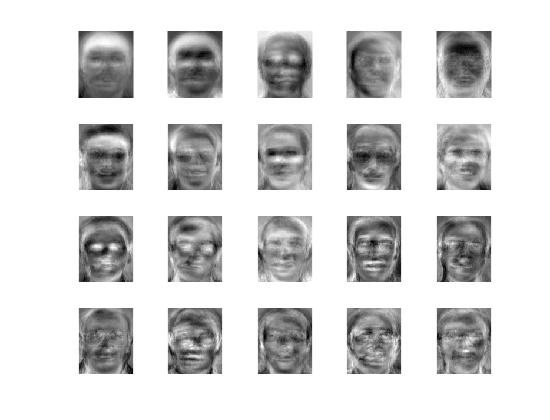
\includegraphics[width=7in]{face.jpg}
\end{figure}


\end{document}

%%% Local Variables: 
%%% mode: latex
%%% TeX-master: t
%%% End: 
